\section{No rule leads across collections}\label{sec:coll}

Table~\ref{tab:collections2} and Figure~\ref{fig:collections} give the accuracy of every rule on every collection. Three observations organise the rest of the paper.

\begin{table}[t]
\caption{Accuracy (fraction of pairs oriented correctly; exact ties half) of twelve rules on eight collections. All rules see the raw arrays, except that T\"ubingen is dequantised (Section~\ref{sec:rules}). ``--'': not run, or no value for most pairs (TRA on the changepoint collection; PDM and the first compression implementation only on the original collections). ``Walks (19)'' contains all $19$ untouched recordings ($486$ pairs; the $122$ pairs of ``walks'' come from five of them). The new collections have $8$, $7$ and $4$ distinct edges; intervals that account for clusters are in Appendix Table~\ref{tab:collections_ci}.}
\label{tab:collections2}
\small
\setlength{\tabcolsep}{3.2pt}
\begin{tabular}{@{}lcccccccc@{}}
\toprule
Rule & T\"ub. & iid & walks & Walks & Sachs & Bern. & Chgpt. & Malus\\
 & (102) & (94) & (122) & (19: 486) & (17) & (16) & (70) & (48)\\
\midrule
IGCI & 0.56 & 0.94 & 0.89 & 0.96 & 0.65 & 1.00 & 1.00 & 0.08\\
RECI & 0.61 & 0.98 & 0.94 & 0.83 & 0.53 & 0.25 & 1.00 & 0.56\\
ANM-HSIC & 0.61 & 0.72 & 0.63 & 0.43 & 0.59 & 0.31 & 0.57 & 0.31\\
Pairwise LiNGAM & 0.61 & 0.78 & 0.71 & 0.67 & 0.53 & 0.88 & 0.43 & 0.40\\
PDM & 0.40 & 0.93 & 0.84 & -- & -- & -- & -- & --\\
LOCI & 0.65 & 0.77 & 0.68 & -- & 0.47 & 0.56 & 0.80 & 0.38\\
ANM, Gaussian process & 0.55 & 0.77 & 0.67 & -- & 0.56 & 0.47 & 0.54 & 0.33\\
Compression, floor256 & 0.61 & 0.30 & 0.61 & -- & 0.76 & -- & -- & --\\
Compression, round255 & 0.67 & 0.38 & 0.52 & 0.50 & 0.65 & 0.50 & 1.00 & 0.60\\
TRA & 0.65 & 0.86 & 0.61 & 0.56 & 0.59 & 0.62 & -- & 0.54\\
AVICI & 0.59 & 0.90 & 0.56 & 0.63 & 0.53 & 0.62 & 0.40 & 0.02\\
RESIT & 0.61 & 0.71 & 0.65 & 0.48 & 0.47 & 0.25 & 0.53 & 0.50\\
\bottomrule
\end{tabular}
\end{table}

\begin{figure}[t]
\centering
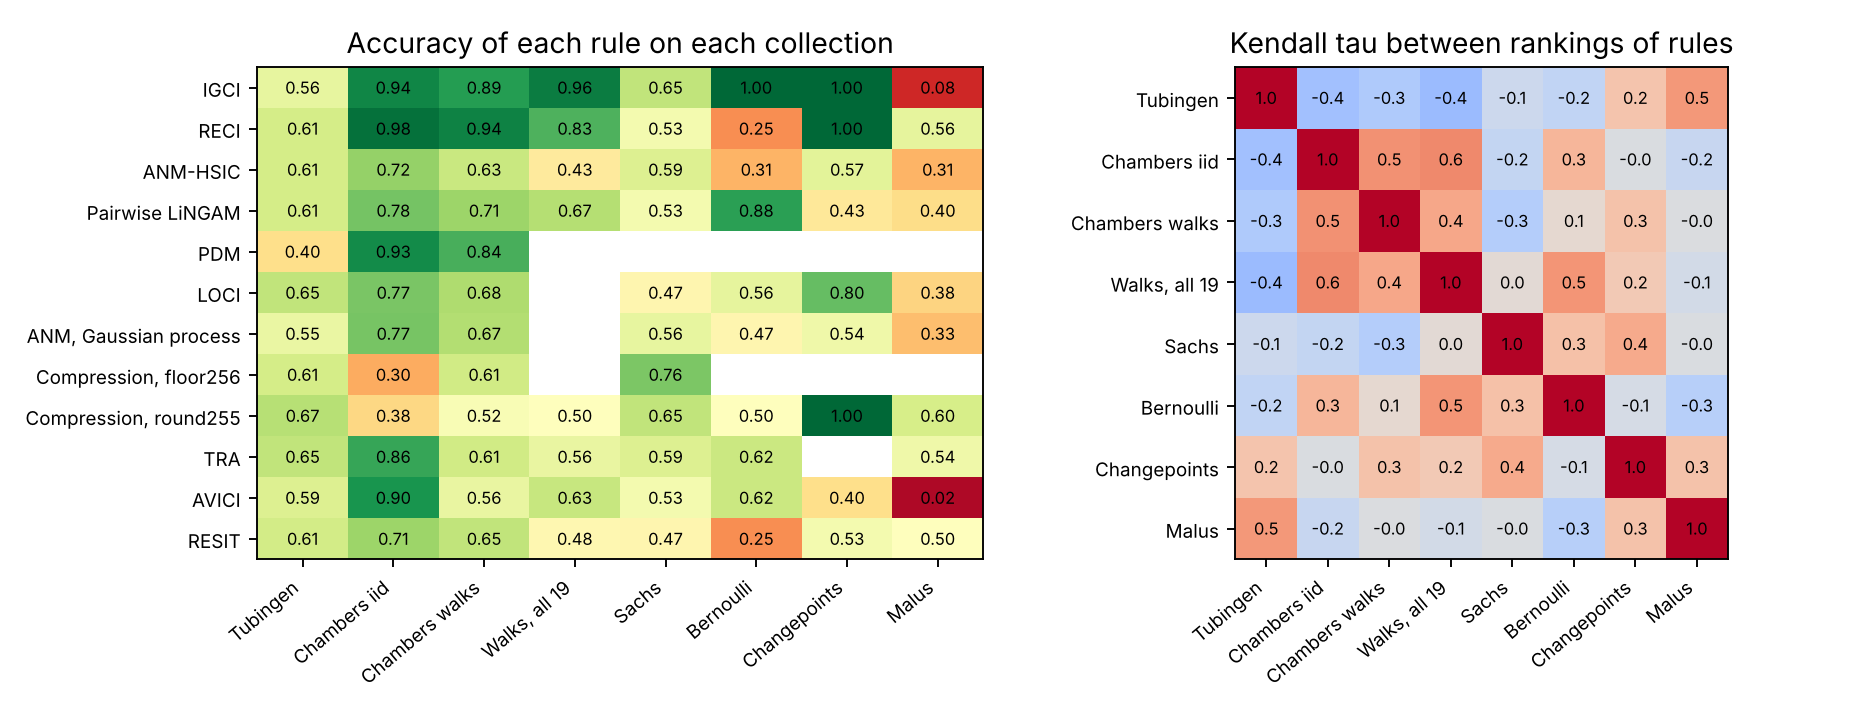
\includegraphics[width=\linewidth]{figs/collections.png}
\caption{Left: accuracy of each rule on each collection. Right: Kendall rank correlation between the orderings of the rules on two collections (rules run on both; at least five).}
\label{fig:collections}
\end{figure}

\paragraph{(1) The leader changes with the collection.} The best rule is round255 compression on T\"ubingen ($66.7\%$; LOCI and TRA at $64.7$ and $64.6\%$) and on the Malus collection ($60.4\%$), RECI on the two chamber collections with independent or random-walk actuators ($97.9\%$ and $94.3\%$), IGCI on all $19$ untouched walk recordings ($95.7\%$; RECI $82.9\%$) and on the Bernoulli collection ($100\%$), the floor256 variant on the $17$ Sachs pairs ($76.5\%$; the round255 one $64.7\%$), and IGCI, RECI and round255 compression together on the changepoint collection ($100\%$). Four of the twelve rules lead at least one collection (counting the two compression implementations separately; the floor256 variant leads Sachs by $13$ against $11$ of $17$ pairs for the round255 one, and the round255 one was chosen to match a published figure, so its leads on T\"ubingen and Malus partly reflect that choice). IGCI is above $70\%$ on five collections and at $8.3\%$ on Malus and $55.9\%$ on T\"ubingen; RECI is above $70\%$ on four; pairwise LiNGAM is above $70\%$ on three (i.i.d.\ $78\%$, walks $71\%$, Bernoulli $88\%$), and no other rule is above $70\%$ on more than two.

\paragraph{(2) Rules that agree on one collection can disagree on the next.} IGCI orients the Bernoulli and the changepoint pairs correctly in every case ($16/16$, $70/70$) and the Malus pairs wrongly in $44$ of $48$. RECI, best or tied-best on three collections, is at $25\%$ on the Bernoulli pairs. The pretrained AVICI model, run on two-variable inputs, is at $90.4\%$ on the i.i.d.\ chambers and at $2.1\%$ on Malus, where it prefers the reverse direction for $47$ of the $48$ pairs. Round255 compression is at $100\%$ on the changepoint pairs, $60.4\%$ on Malus and $38.3\%$ on the i.i.d.\ chambers. The additive-noise rules are never the best: ANM-HSIC is at $43.4\%$ on the $19$ walk recordings (cluster interval $[38,50]$), RESIT at $47.5\%$. With the recordings as clusters, cluster-level sign-flip tests of the difference in accuracy give IGCI above RECI on the $19$ recordings ($p=0.019$), RECI above ANM-HSIC ($p<0.001$), above AVICI and above pairwise LiNGAM ($p<0.001$); on the i.i.d.\ chambers (47 edges as clusters) RECI is above ANM-HSIC ($p<0.001$) and pairwise LiNGAM ($p=0.001$) and IGCI above ANM-HSIC ($p=0.012$), but IGCI and RECI are not separated ($p=0.63$); with five recordings the smallest attainable $p$ is $0.0625$. The ordering of the leaders on the walks is therefore resolved: IGCI $95.7\%$ ($[91,99]$), RECI $82.9\%$ ($[79,87]$), pairwise LiNGAM $67.1\%$, AVICI $63.4\%$, TRA $55.6\%$, round255 compression $50.2\%$, RESIT $47.5\%$, ANM-HSIC $43.4\%$; the between-recording standard deviation of a rule's accuracy is $0.08$ to $0.15$.

\paragraph{(3) Rankings of rules do not clearly transfer.} The Kendall correlation between the ordering of the rules on T\"ubingen and on the i.i.d.\ chambers is $-0.38$, against the walk pairs $-0.30$ ($-0.42$ for all $19$ recordings), against Sachs $-0.12$ and Bernoulli $-0.19$; it is positive against the changepoints ($+0.24$) and Malus ($+0.51$). The chamber collections agree with each other (i.i.d.\ against walks $+0.53$, against all $19$ recordings $+0.57$). With a permutation test over the rules none of the T\"ubingen correlations is distinguishable from zero ($p=0.06$ to $0.68$): the T\"ubingen accuracies span about twelve points with intervals of $\pm0.10$, so the ordering of the rules on that collection is mostly noise. The full matrix with permutation $p$-values is in Appendix Table~\ref{tab:kendall}. What it does not show is a shared ranking: a rule that leads T\"ubingen says little, in either direction, about a collection from a device with a documented graph. The two compression variants and PDM are counted as rules, and the i.i.d.\ and walk collections come from the same devices.

\paragraph{Cautions.} The cluster-bootstrap intervals of Appendix Table~\ref{tab:collections_ci} (clusters: $47$ edges for the i.i.d.\ chambers, $5$ and $19$ recordings for the two walk collections, $8$, $7$ and $4$ edges) are close to the exact intervals for the i.i.d.\ chambers (RECI $0.98$ [$0.94$, $1.00$]) and for T\"ubingen but are degenerate when a rule is right on every cluster (RECI on the changepoints, $1.00$ [$1.00$, $1.00$]) and unreliable with four to eight clusters; their purpose is to show how few independent units the new collections contain. The Bernoulli, changepoint and Malus collections consist of $8$, $7$ and $4$ distinct edges, repeated across seeds or experiments, with the same cause variable (\texttt{load\_in}, or the two polarisers); they are small, correlated sets of regimes, not samples of mechanisms, and we use them as such. Sachs has $17$ pairs. The T\"ubingen collection mixes pairs from several fields and its weights downweight groups of similar pairs; unweighted accuracy is used here unless stated. IGCI's results depend on how ties are handled (Section~\ref{sec:ties}); the numbers here are for the raw arrays. The T\"ubingen arrays are dequantised, a convention that also matters: on raw T\"ubingen arrays IGCI is at $63.8\%$ on average over the protocol configurations of Section~\ref{sec:protocol_multiverse} (against $52.4\%$ dequantised), above RECI, so the T\"ubingen column and its Kendall correlations depend on this convention. The point estimates behind ``the leader changes'' are not all resolved: round255 compression leads T\"ubingen by one pair over LOCI ($p=0.88$), Malus by three points with four clusters, and Sachs the floor256 variant by $13$ against $11$ of $17$ pairs. The $28$ Kendall correlations are uncorrected for multiplicity: one has a raw permutation $p<0.05$ (i.i.d.\ against walks, $0.02$) and none survives a Holm correction (smallest adjusted $p=0.49$), so no statement of agreement or disagreement between collections is supported at the level of the rank correlations. The i.i.d., walk, Bernoulli, changepoint and Malus collections are best read as case studies of regimes of two devices rather than as samples of mechanisms; in them the cause is an experimenter-set actuator and the effect a sensor, a feature of the experimental design, so a marginal cue for ``actuator'' versus ``sensor'' is not evidence about cause and effect in general.
